\chapter{主要组织相容性抗原}
\begin{framed}
\noindent\textbf{【知识体系】}
\begin{center}
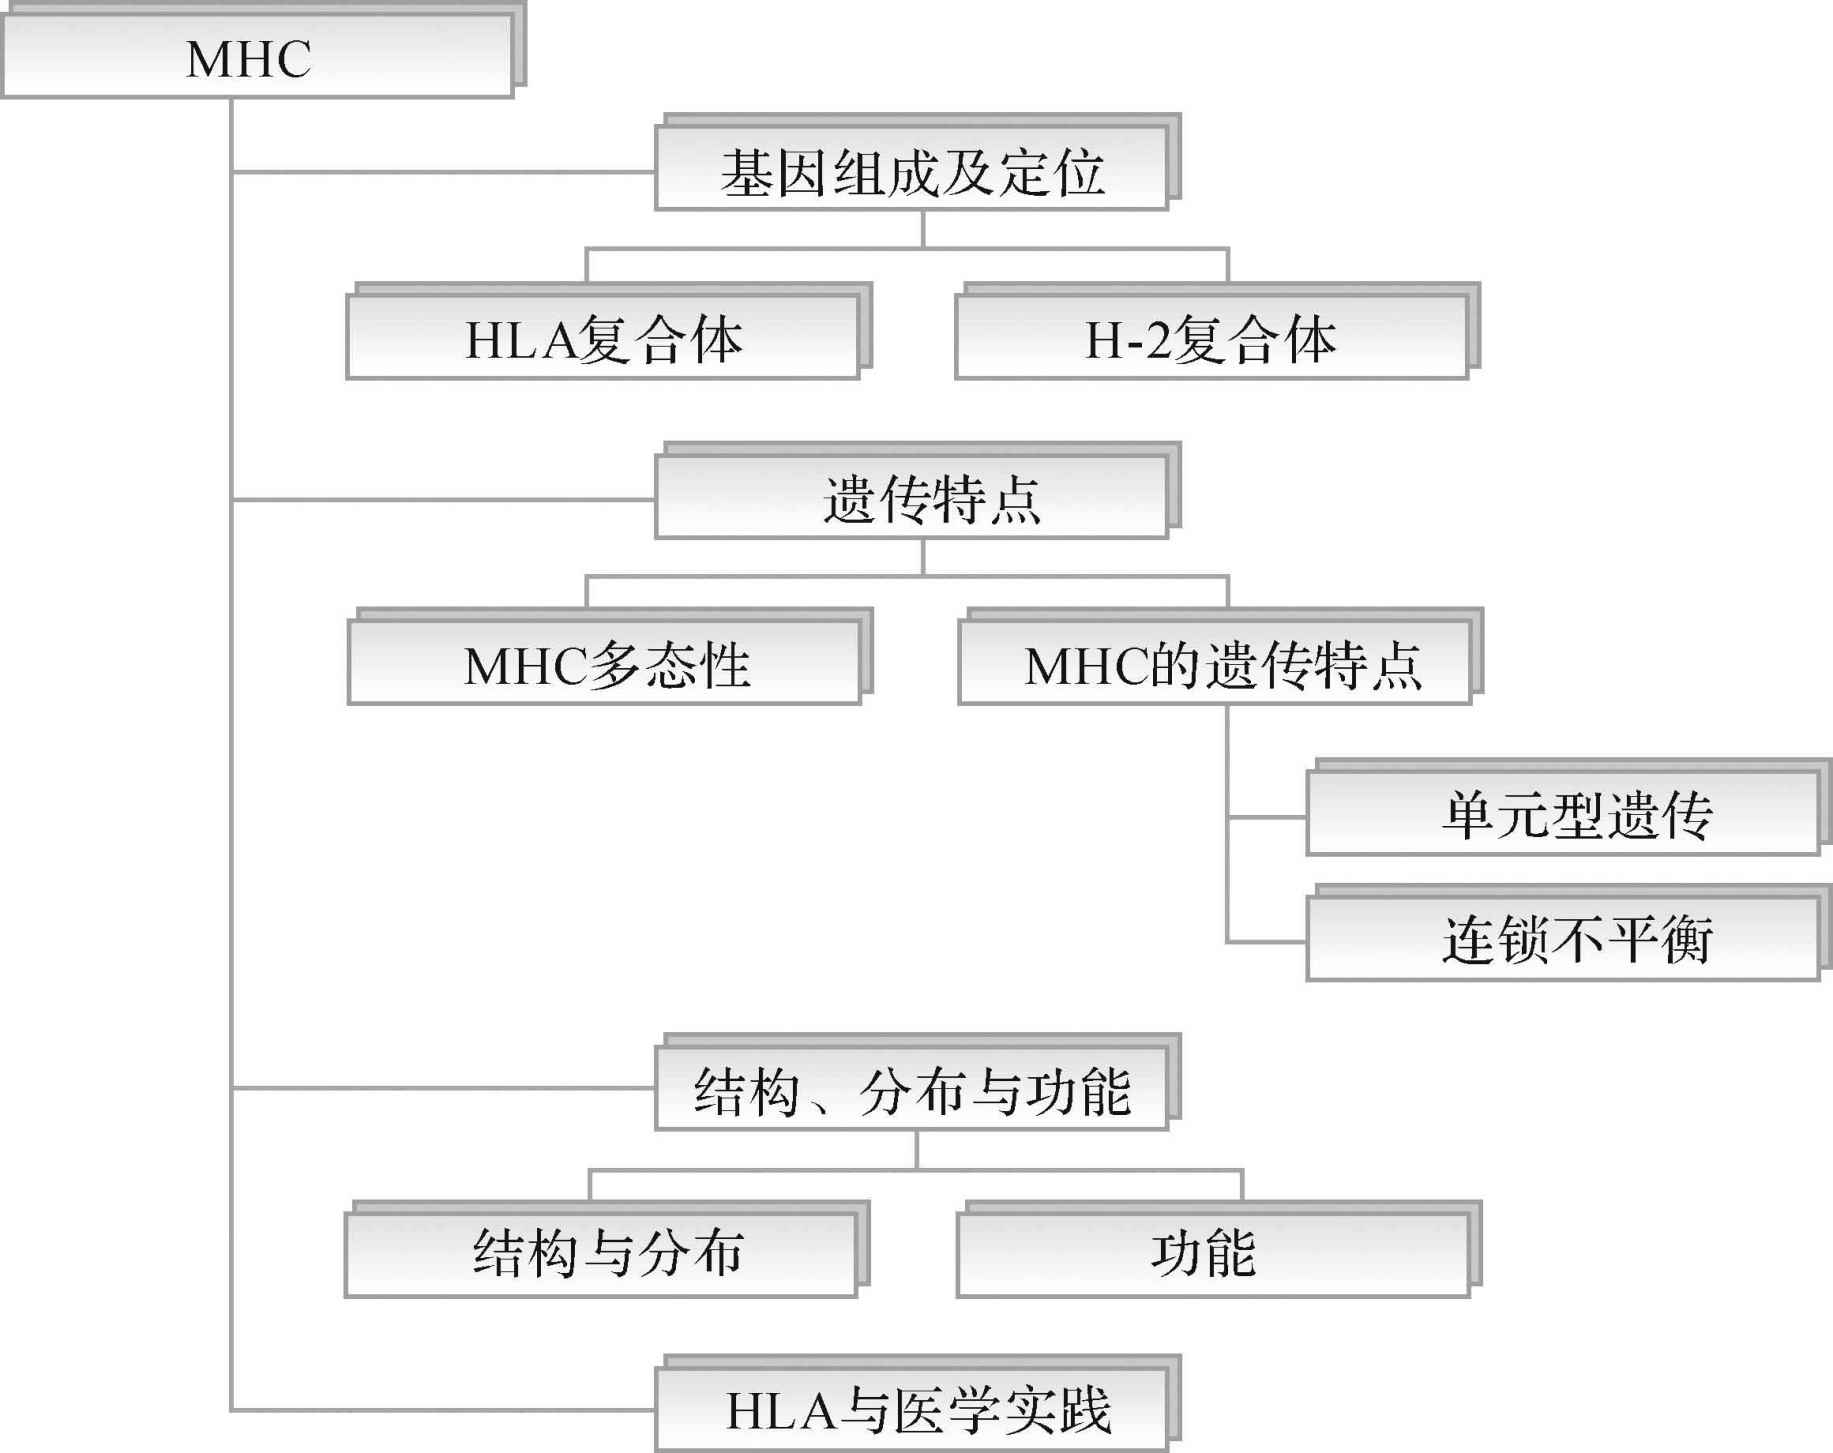
\includegraphics{./images/Image00101.jpg}
\end{center}
\noindent\textbf{【课前思考】}

每个个体独有、在器官移植及亲子鉴定中起主要作用的是什么成分?它有什么结构?为什么它有多样性?有哪些生物学功能?

\noindent\textbf{【本章重点】}

1.MHC概念,MHC-Ⅰ类和Ⅱ类分子的结构、分布;

2.MHC的生物学功能。

\noindent\textbf{【教学目标】}

1.掌握MHC/HLA的概念、MHC-I、MHC-II分子的分布及其生物学功能;

2.熟悉MHC分子抗原递呈作用的分子机制。
\end{framed}

主要组织相容性复合体(major histocompatibility complex,MHC)
即编码主要组织相容性抗原的一组紧密连锁的基因群,定位于动物与人某对染色体的特定区域,呈高度多态性。MHC的编码产物即MHC分子或MHC抗原,其表达于不同细胞表面,主要功能是参与抗原递呈、制约细胞间相互识别及诱导免疫应答。

在人或同种不同品系动物个体间进行组织移植时,可因二者组织细胞表面同种异型抗原存在差异而发生排斥反应。这种抗原称组织相容性Ag或移植Ag。其中可诱导迅速而强烈排斥反应者被称为主要组织相容性抗原,其编码基因即主要组织相容性(基因)复合体(MHC);可诱导较弱排斥反应的被称为次要组织相容性抗原,其编码基因为次要组织相容性(基因)复合体(minor
histocompatibility
complex,mHC)。已证实,MHC的生物学意义远超出移植免疫范畴,其编码产物是参与免疫应答的关键成分,但MHC的命名则沿用至今。

Gorer于1936年发现了小鼠的MHC,即H-2,继之Dausset于50年代末确定了人类MHC,即HLA(human
leukocyte
antigen)(图\ref{fig7-1})。近年来,转基因动物、异种移植、克隆动物/器官等领域的飞速发展进一步促进了对多种哺乳动物MHC的研究。不同种类哺乳动物MHC及其编码产物的名称各异,但其基因结构、产物及功能均有相似之处。习惯上,MHC(或HLA复合体)一般指基因,MHC分子/抗原(或HLA分子/抗原)则指编码产物,有不同的命名(表\ref{tab7-1})。

小鼠的MHC:H-2复合体位于第17号染色体上。

人类的MHC:HLA复合体位于第6号染色体上。

\begin{figure}[!htbp]
 \centering
 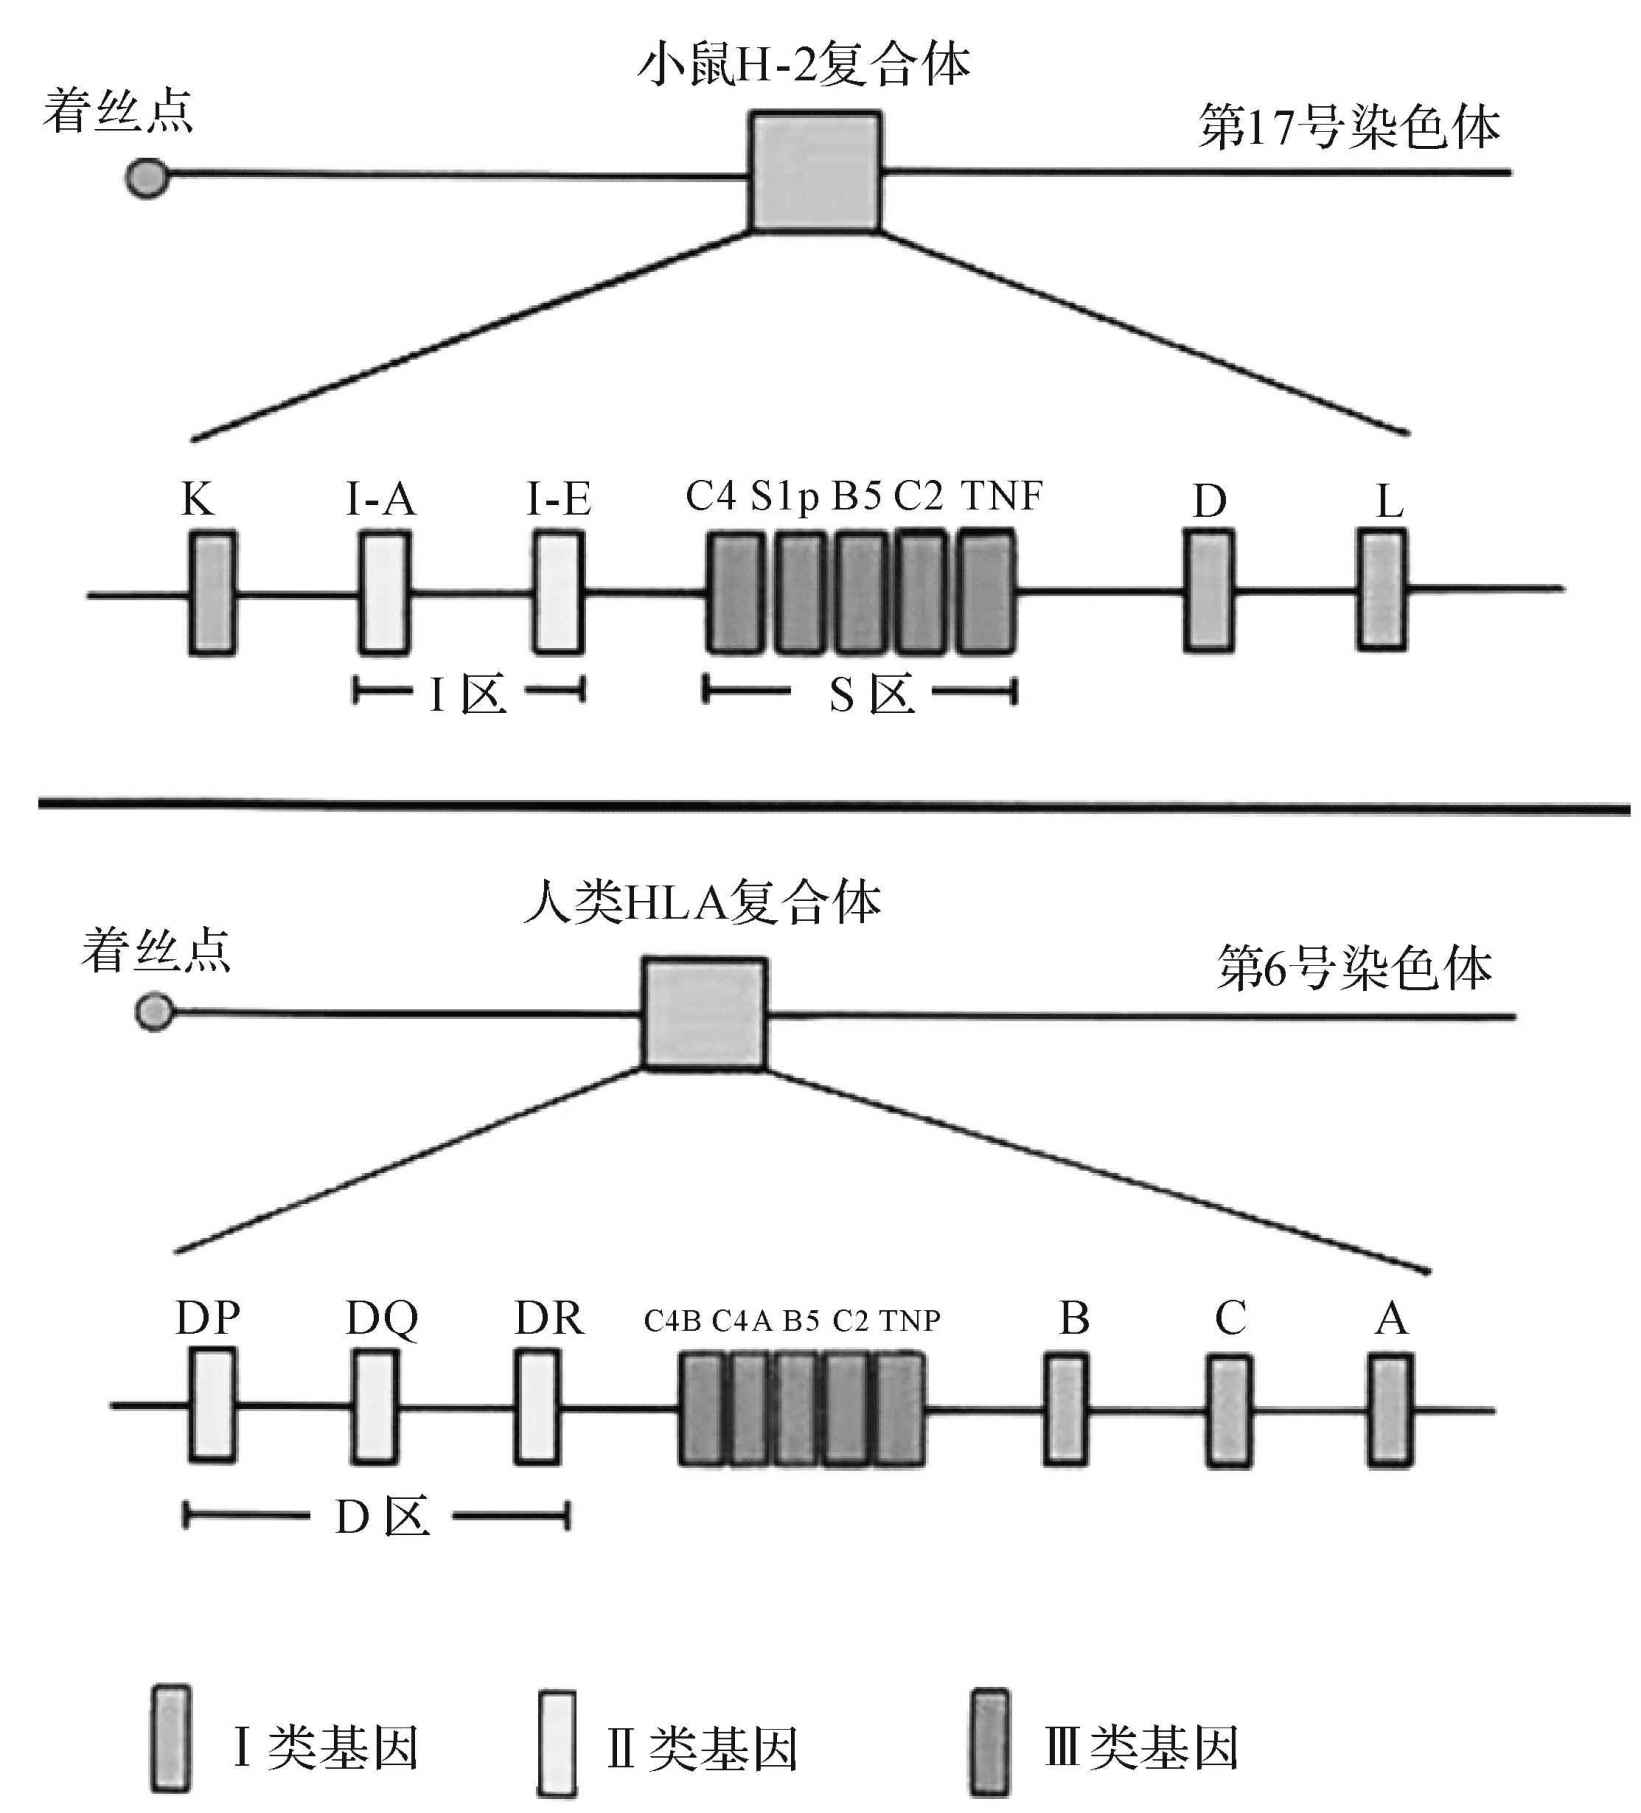
\includegraphics{./images/Image00102.jpg}
 \captionsetup{justification=centering}
 \caption{H-2和HLA的结构示意图}
 \label{fig7-1}
  \end{figure} 

\begin{longtable}[]{@{}llllll@{}}
    \caption{不同动物的MHC名称}
    \label{tab7-1}\\
\toprule
种属 & 人 & 小鼠 & 大鼠 & 黑猩猩 & 鸡\tabularnewline
\midrule
\endhead
名称 & HLA & H-2 & H-1 & ChLA & B\tabularnewline
\bottomrule
\end{longtable}

\section{MHC的基因组成及定位}

MHC基因复合体的特点之一为多基因性,即HLA复合体的基因数量和结构具有多样性。众多MHC基因依其编码分子的特性而分为MHC-Ⅰ类、-Ⅱ类及-Ⅲ类基因。


\subsection{人类HLA复合体}

人类MHC亦称HLA复合体,位于第6号染色体短臂。HLA复合体的特点之一是其多基因性,目前已鉴定出100余个基因座位。诸多HLA基因座按其定位和特点,可分为三类(图\ref{fig7-2})。

\begin{figure}[!htbp]
 \centering
 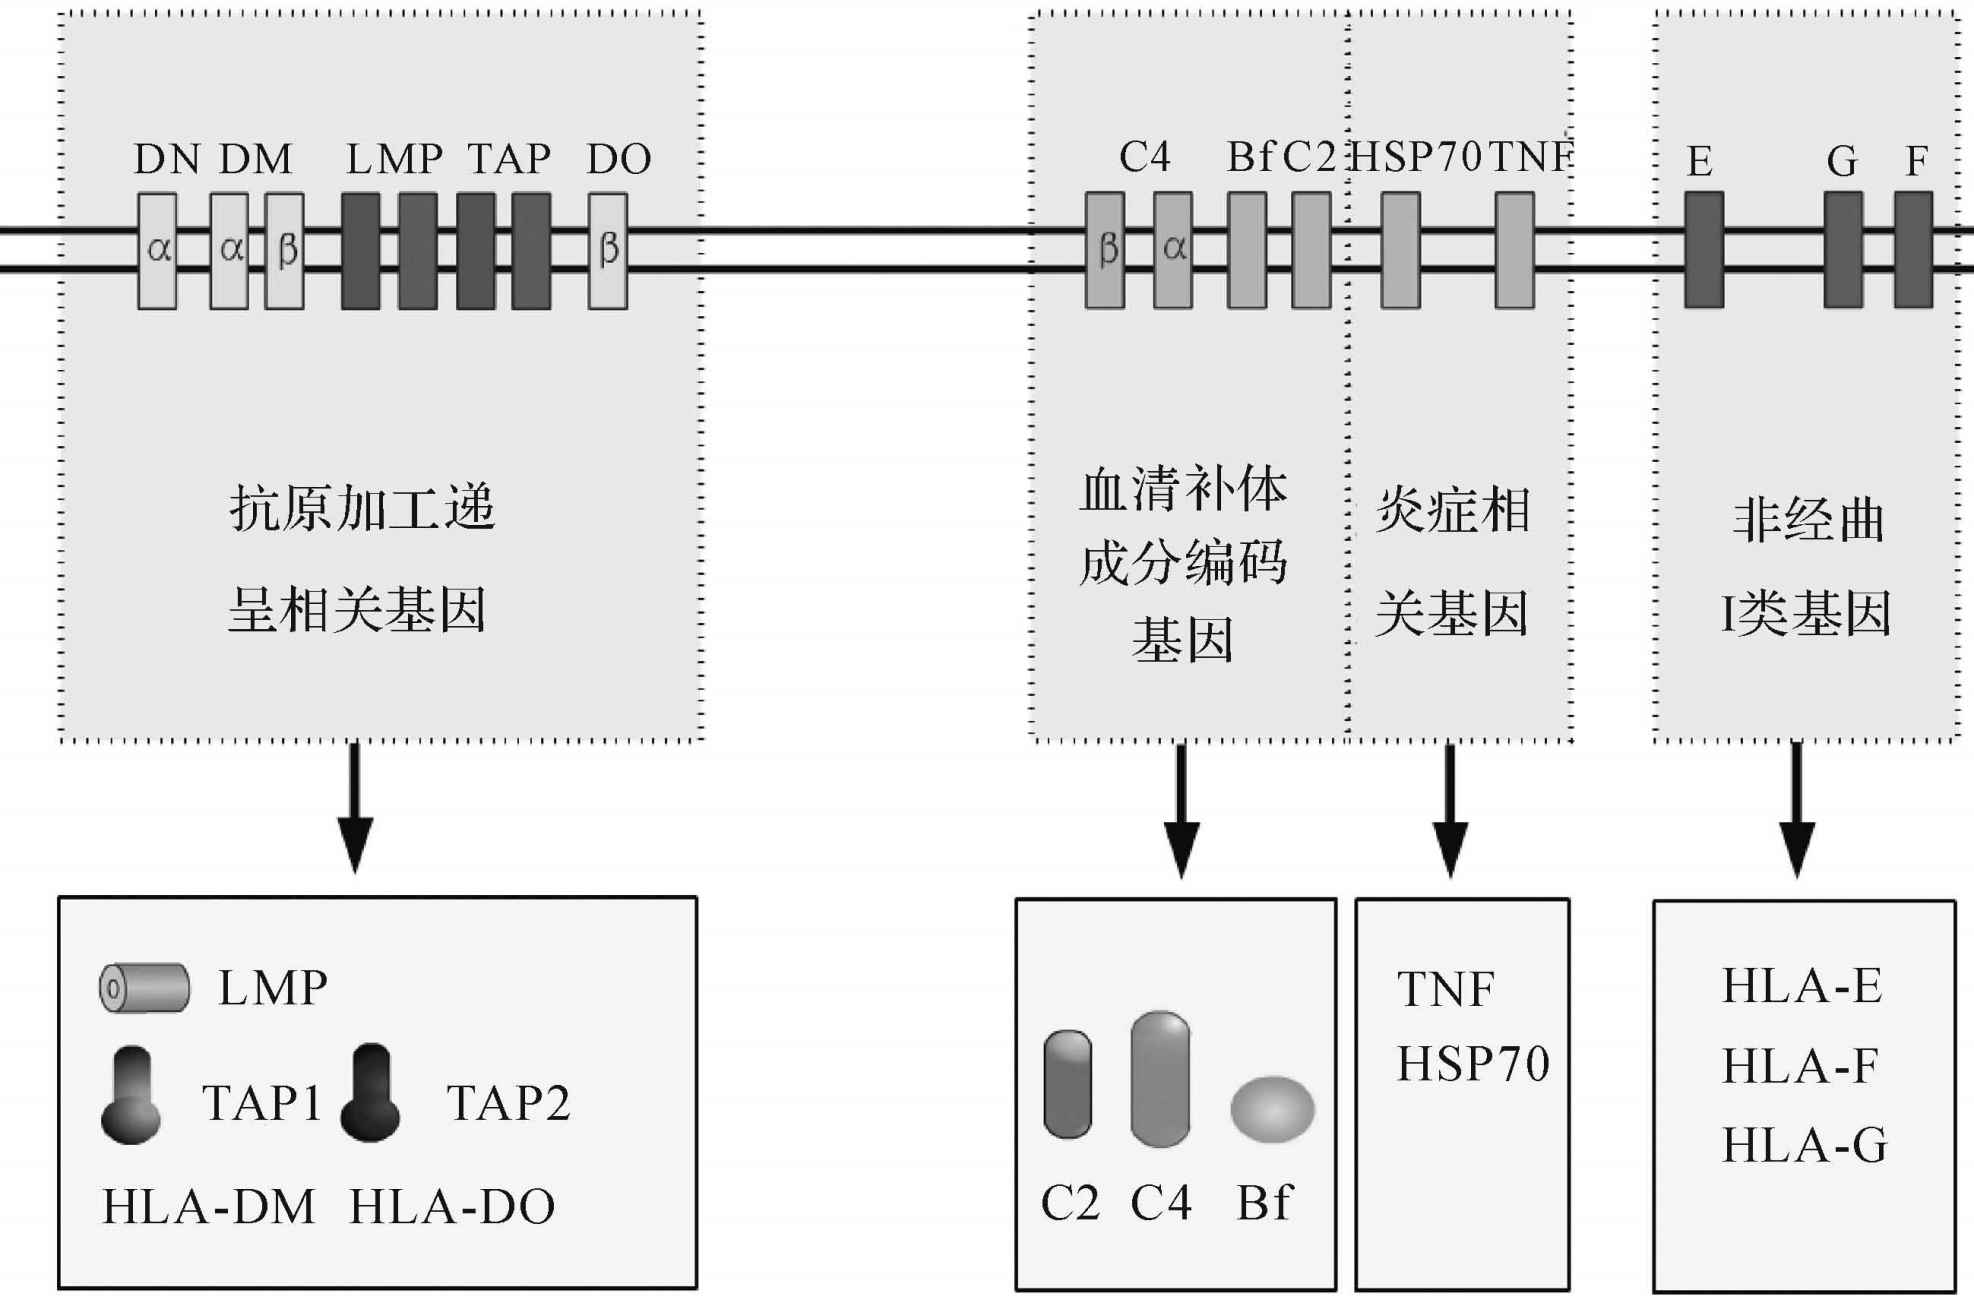
\includegraphics[width=.6\textwidth]{./images/Image00103.jpg}
 \captionsetup{justification=centering}
 \caption{免疫功能相关基因及其相关编码产物}
 \label{fig7-2}
  \end{figure} 

1.HLA-Ⅰ类基因:经典的HLA-Ⅰ类基因包括HLA-B、-C、-A,它们具有多态性,组织分布广泛,主要生物学功能是参与递呈内源性抗原。

非经典Ⅰ类基因包括HLA-E、HLA-G及HLA-F基因。这些基因多态性有限,选择性表达于机体某些组织,其生物学功能尚未完全阐明。

2.HLA-Ⅱ类基因:经典的HLA-Ⅱ类基因包括HLA-DP、-DQ和-DR,它们也具有高度多态性,主要生物学功能是递呈外源性抗原。

非经典Ⅱ类基因包括低分子量多肽(low molecular-weight
polypeptide,LMP)基因、抗原加工相关转运体(transporter associated with
antigen processing,TAP)基因、TAP相关蛋白(TAP-associated
protein)基因(编码产物亦称为tapasin)、HLA-DM基因及HLA-DO基因等,这些基因编码产物的主要功能是参与抗原加工和转运。

低分子量多肽基因LMP:包括LMP2、LMP7座位,蛋白酶体相关基因(proteasome-related
gene)编码蛋白酶体相关成分,参与内源性抗原的酶解。

抗原加工相关转运体基因TAP:包括TAP1、TAP2座位,编码产物TAP(transporter
of antigenic
peptides)位于内质网膜上,参与对内源性抗原的转运,使其进入内质网腔。

HLA-DM基因:包括DMA、DMB座位,产物参与APC对外源性抗原的加工递呈,帮助溶酶体中的抗原片段进入MHC
II类分子的抗原结合槽。

HLA-DO基因:包括DOA、DOB座位,编码的DO分子是DM功能的负向调节蛋白。

3.HLA-Ⅲ类基因:位于Ⅰ类与Ⅱ类基因之间,包括编码补体C4b、C4a、C2和Bf的基因,以及编码炎症相关分子、TNF、I-κB(转录调节分子)、热休克蛋白(heat
shock protein 70,HSP70)等产物的基因。


\subsection{小鼠H-2复合体}

小鼠H-2复合体与人类HLA复合体在基因结构、编码产物分布及功能等方面均有诸多对应与相似之处,故小鼠成为研究人类MHC的最佳模型和有效工具(图\ref{fig7-3})。迄今对MHC的认识主要得益于对小鼠H-2的研究。

小鼠H-2复合体定位于第17号染色体,依次为K、I、S、D/L四个区域。根据编码分子的特征可将H-2复合体分为3类基因:Ⅰ类基因包括K、D、L三个座位或区域;Ⅱ类基因又称为I区基因,位于H-2复合体的免疫应答区(immune
response
region),由I-A和I-E亚区组成,参与免疫应答的遗传控制及调节;Ⅲ类基因为编码血清补体成分及TNF等。

\begin{figure}[!htbp]
 \centering
 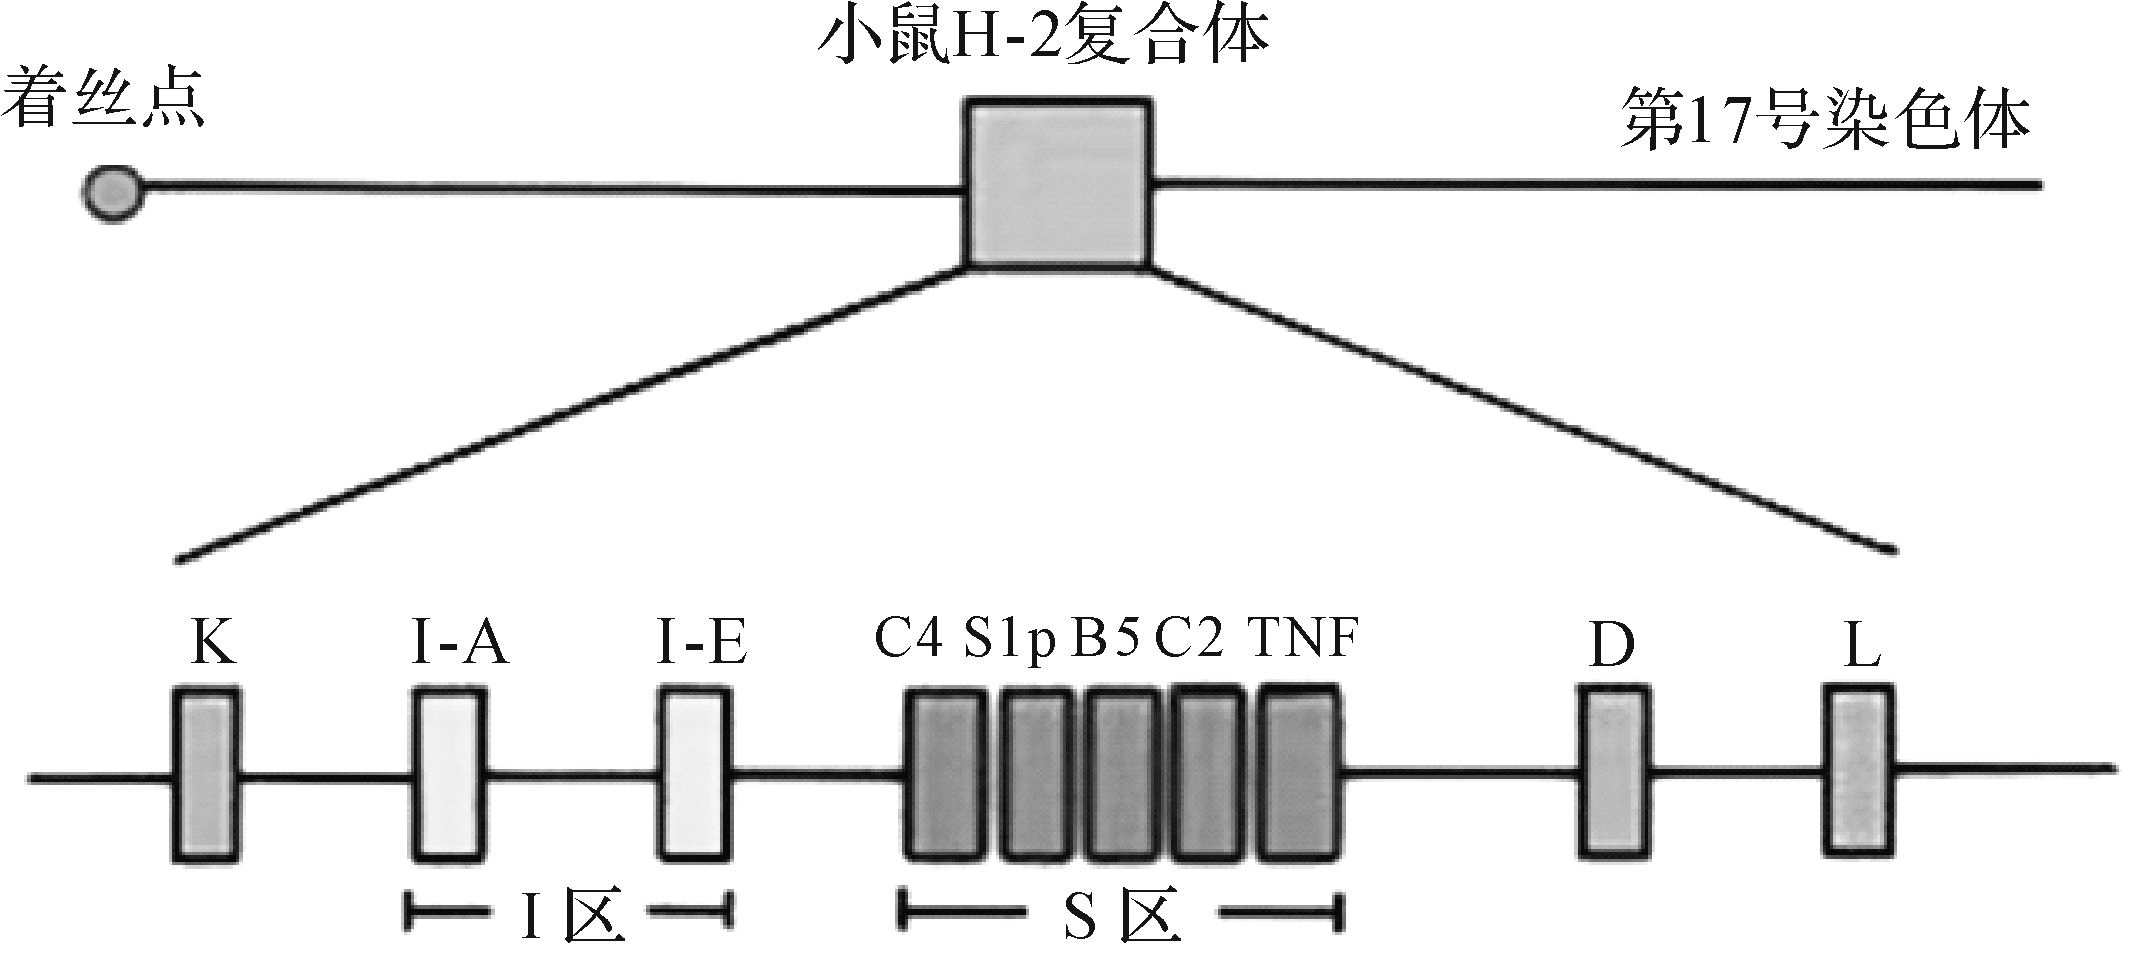
\includegraphics{./images/Image00104.jpg}
 \captionsetup{justification=centering}
 \caption{H-2的结构示意图}
 \label{fig7-3}
  \end{figure} 

\section{MHC的遗传特点}


\subsection{MHC多态性}

对同一个体而言,染色体上任一基因座位只能有两个等位基因,分别来自父、母的同源染色体。但在随机婚配的群体中,同一基因座位可能存在两个以上等位基因,此现象被称为多态性(polymorphism)。需强调的是:多态性乃群体的概念,指群体中不同个体同一基因座位上的基因存在差别。MHC是哺乳动物体内具有最复杂多态性的基因系统。

(一)MHC多态性的产生机制

MHC的多态性的发生机制主要是MHC基因座存在复等位基因及其共显性表达。

1.复等位基因 (multiple
allele):在群体中,位于同一基因座的不同基因系列即为复等位基因。MHC复合体的多数基因座均有复等位基因,此乃形成MHC基因多态性最根本的原因。目前,HLA复合体中已发现的复等位基因达1556个,抗原特异性数为164个。

2.共显性(co-dominant)表达:共显性即两条染色体同一基因座每一等位基因均为显性基因,均能编码特异性抗原。共显性表达极大增加了MHC抗原系统的复杂性,此乃MHC表型多态性的重要机制。

MHC基因和编码分子的命名原则:星号(*)前为基因座,星号后为等位基因。根据等位基因的结构,通常再分成若干主型。例如:MHC-A*0103代表MHC-Ⅰ类基因A座位第1主型的3号基因。该命名系统为有待发现的基因座和等位基因预留出了位置。

MHC编码产物亦称为MHC分子或抗原。目前已鉴定出的MHC分子种类数少于等位基因的数目。Dw代表激发同种异体淋巴细胞增殖的淋巴细胞激活决定簇
(LAD),是DR、DQ等II类基因产物效应的总和,但不存在单独的Dw基因座。

(二)MHC多态性的意义

1.赋予种群适应多变的环境条件:MHC多态性使种群具有极大的基因储备,造就了对特定抗原(病原体)应答能力(易感性)各异的个体,保证在群体水平能应付多变的环境条件及各种病原体的侵袭,从而有利于种群的生存和延续。

2.实现对机体免疫应答的遗传控制:MHC基因多态性使其编码产物分子结构(主要是抗原结合槽)各异,从而决定其与特定抗原肽结合的选择性及亲和力。由此,个体的遗传背景决定了其对特定抗原是否产生应答,以及应答水平的强弱。

3.使MHC成为个体的终生遗传标志:由于MHC的高度多态性,无亲缘关系的个体间出现MHC型别全相同者的几率极低,故MHC型别可视为个体的终生遗传标志。这一特征被用于疾病研究和法医学的个体识别。

4.增加了寻找合适同种器官移植供者的难度:由于MHC基因型和表型均具有极为复杂的多态性,故在无血缘关系的人群中一般难以找到MHC型别完全相同的个体,从而极大增加了临床上寻找合适器官移植供者的难度,尤其成为开展造血干细胞移植的障碍。为此,目前国内外均已着手建立造血干细胞捐赠者资料库,以有助于筛选出MHC全相同的无关供者。


\subsection{MHC的遗传特点}

(一)单元型遗传

连锁在一条染色体上的若干基因座,其等位基因的组合构成单元型(haplotype)。单元型是将MHC遗传信息传给子代的基本单位,在遗传过程中一般不发生同源染色体互换。人类细胞含两个同源单元型,组成两个单元型的全部等位基因构成MHC基因型(genotype),其编码产物为MHC表型(phenotype)。

粗略估算,人群中的单元型数目超过5×10\textsuperscript{8}
,而由两个单元型所决定的表型更是不计其数。人类细胞内的两个同源染色体分别来自父母,故比较两个同胞间单元型型别,存在三种可能性:两个单倍体型均相同,其几率为25\%;两个单元型均不同,其几率亦为25\%;有一个单元型相同,其几率为50\%。上述遗传规律在器官移植供者的选择及法医亲子鉴定中得到应用。

(二)连锁不平衡

MHC等位基因的频率,指群体中携带某一等位基因的个体数目与携带该基因座各等位基因个体数目总和的比例。由于MHC复合体的各座位紧密连锁,若各座位的等位基因均随机组合构成单元型,则某一单元型的频率应等于组成该单元型各等位基因频率的乘积。但实际上,MHC各等位基因并非完全随机组成单元型。已发现,某些等位基因比其他等位基因更多或更少地连锁在一起,即出现连锁不平衡(linkage
disequilibrium)。例如,北欧白种人HLA-A1和HLA-B8的出现频率分别为0.17和0.11,若随机组合,其单元型A1-B8连锁的预期频率应为0.17×0.11=0.019,而实测值为0.088,二者的差额(0.088-0.019=0.069)即为连锁不平衡参数。由于连锁不平衡,使得人群中实际存在的单元型数目少于理论值,且某些单元型在群体中可呈现较高频率(图\ref{fig7-4})。

\begin{figure}[!htbp]
 \centering
 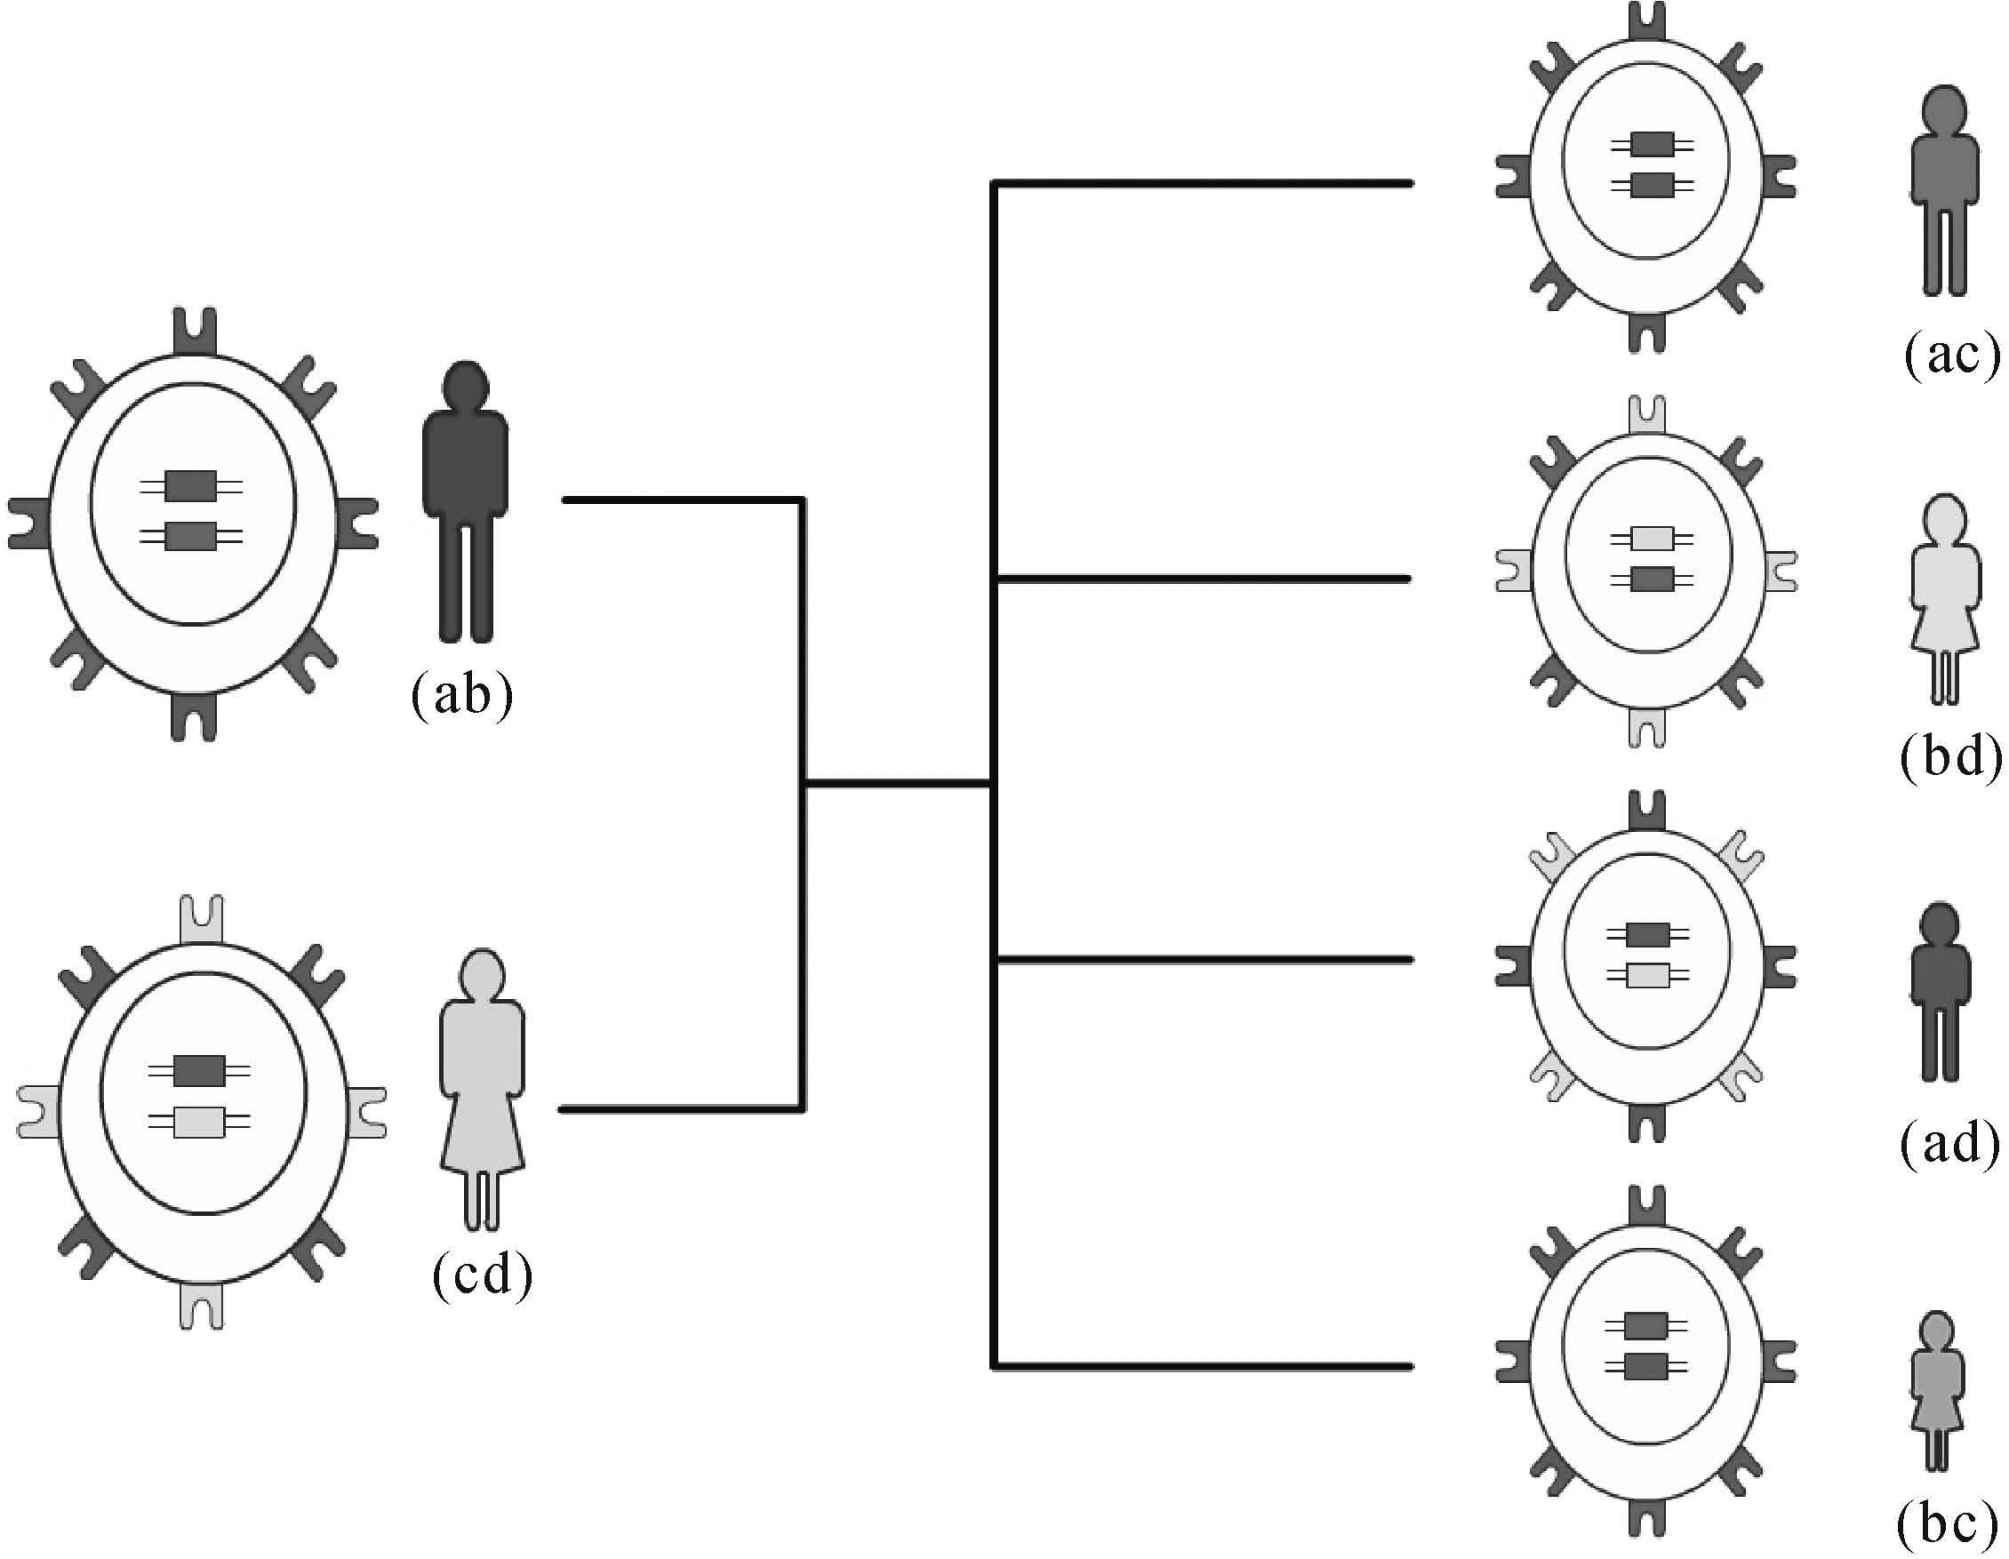
\includegraphics{./images/Image00105.jpg}
 \captionsetup{justification=centering}
 \caption{HLA的单元型遗传示意图}
 \label{fig7-4}
  \end{figure} 

\section{MHC分子结构、分布与功能}


\subsection{MHC分子的结构与分布}

(一)MHC-Ⅰ类分子的结构与分布

MHC-Ⅰ类分子属糖蛋白,由一条重链(跨膜成分,44kD
367个aa)和一条轻链(非跨膜成分,12kD 99个aa
)以非共价键连接而成,其结构示意图如图\ref{fig7-5}所示。具多态性的重链也称为α链,包括α1、α2与α3结构域,其中α1、α2结构域共同构成抗原(肽)结合槽;轻链即β-2微球蛋白(microglobulin,β2m),乃由位于第15号染色体的非MHC基因所编码,与重链的α3同属免疫球蛋白超家族。β2m无多态性,其以非共价键与α链胞外段相互作用,有助于维持Ⅰ类分子天然构型的稳定性。

\begin{figure}[!htbp]
 \centering
 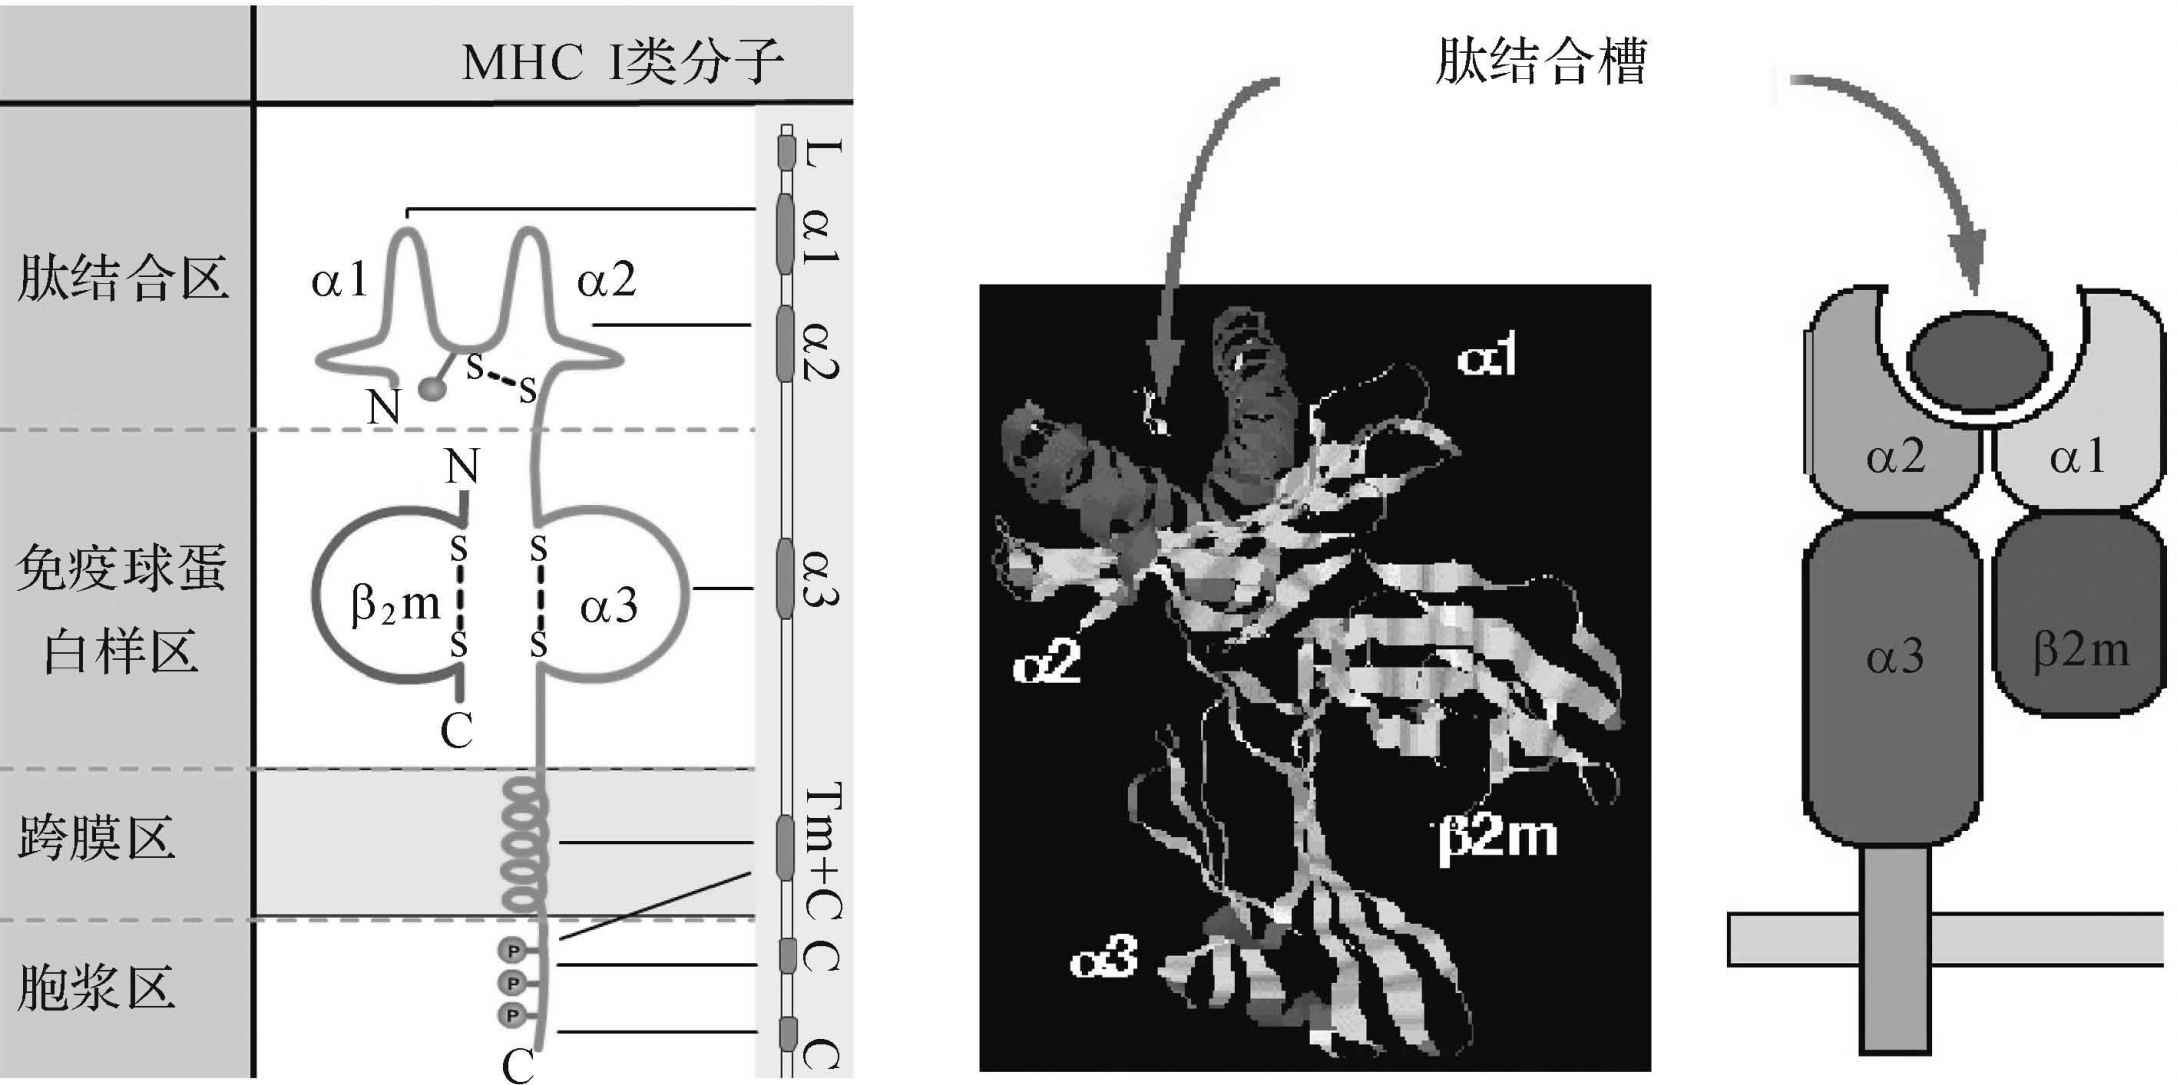
\includegraphics{./images/Image00106.jpg}
 \captionsetup{justification=centering}
 \caption{MHC-Ⅰ类分子结构示意图}
 \label{fig7-5}
  \end{figure} 

Ⅰ类分子分四个区:

(1)肽结合区:
位于N端,有α1、α2两个功能区。含有与Ag结合的部位,是同种异型Ag决定簇存在的部位。

(2)Ig 样区:重链α3、β2 的微球蛋白,α3有90个aa与CD8结合,起黏附作用。

(3)跨膜区:25个氨基酸形成α-螺旋,使Ⅰ类分子固定在细胞膜上。

(4)胞浆区:30个氨基酸,含较多苏氨酸、酪氨酸、丝氨酸,发生磷酸化。

借助X光衍射技术分析Ⅰ类分子空间结构,发现其重链胞外段存在一底部由8条反向平行β片层、边缘由2个α螺旋构成的抗原结合槽,可容纳含8~10个氨基酸残基(或稍长)的多肽片段。抗原结合槽中关键位点的氨基酸残基不同,导致抗原结合槽精细结构、电荷分布各异,从而形成
MHC的多态性,以及I类分子与抗原肽结合的相对专一选择性和亲和力。

MHC-Ⅰ类分子主要分布于机体所有有核细胞表面(包括血小板和网织红细胞),以淋巴细胞表面Ⅰ类分子的密度最大,其次为肾、肝及心脏,密度最低的为肌肉和神经组织。此外,血清、初乳及尿液中还存在可溶性的Ⅰ类分子。

(二)MHC-Ⅱ类分子的结构与分布

MHC-Ⅱ类分子属糖蛋白,乃由α(32-34kD)和β(29-32
kD)两条肽链以非共价键连接而成,如图\ref{fig7-6}所示。如同Ⅰ类分子,Ⅱ类分子也属免疫球蛋白超家族,但其两条链均为跨膜成分。Ⅱ类分子的抗原结合槽为开端结构,故可结合较长(约13~17个氨基酸残基)肽段。Ⅱ类分子分为四个区:

(1)肽结合区(α1,β1):两条螺旋末端开放,可结合14-18个氨基酸,最长可达30个氨基酸。

(2)Ig 样区(α2,β2):与CD4结合。

(3)跨膜区:25个疏水性氨基酸。

(4)胞浆区:10-15个氨基酸。

MHC-Ⅱ类分子仅表达于专职抗原递呈细胞(B细胞、巨噬细胞、树突状细胞、朗格汉斯细胞)以及活化的T细胞和胸腺上皮细胞等表面。

\begin{figure}[!htbp]
 \centering
 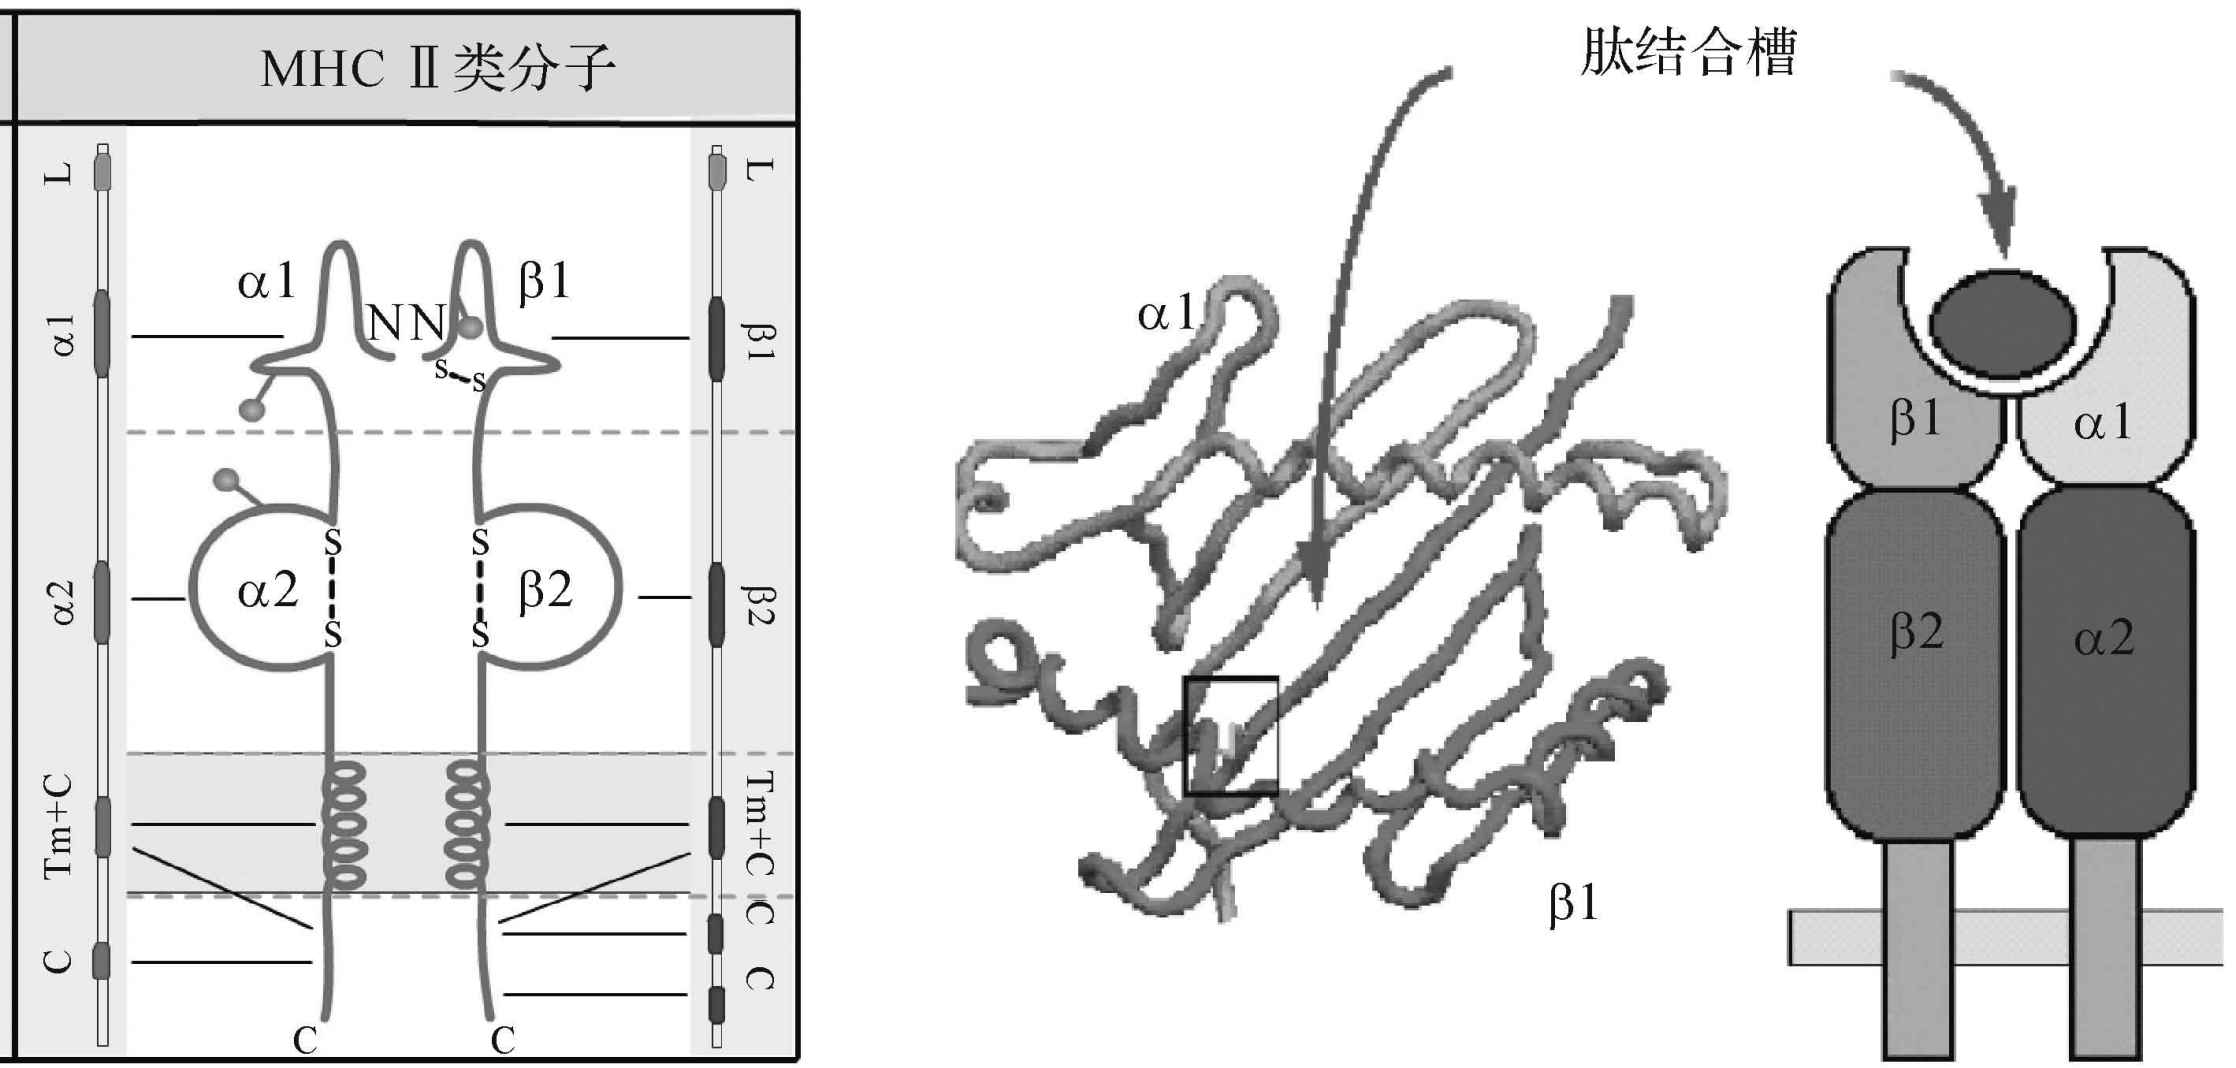
\includegraphics{./images/Image00107.jpg}
 \captionsetup{justification=centering}
 \caption{MHC-Ⅱ类分子结构示意图}
 \label{fig7-6}
  \end{figure} 


\subsection{MHC分子的功能}

(一)参与加工与递呈抗原

MHC-Ⅰ类分子和Ⅱ类分子分别参与对内源性和外源性抗原的加工和递呈,如图\ref{fig7-7}所示。内源性或外源性抗原被加工成为肽段,嵌入MHC-Ⅰ(或Ⅱ)类分子抗原结合槽中,形成抗原肽/MHC-Ⅰ(或Ⅱ)类分子复合物,进而表达于抗原递呈细胞表面供CD8\textsuperscript{+}
T或CD4\textsuperscript{+} T细胞的TCR识别。

\begin{figure}[!htbp]
 \centering
 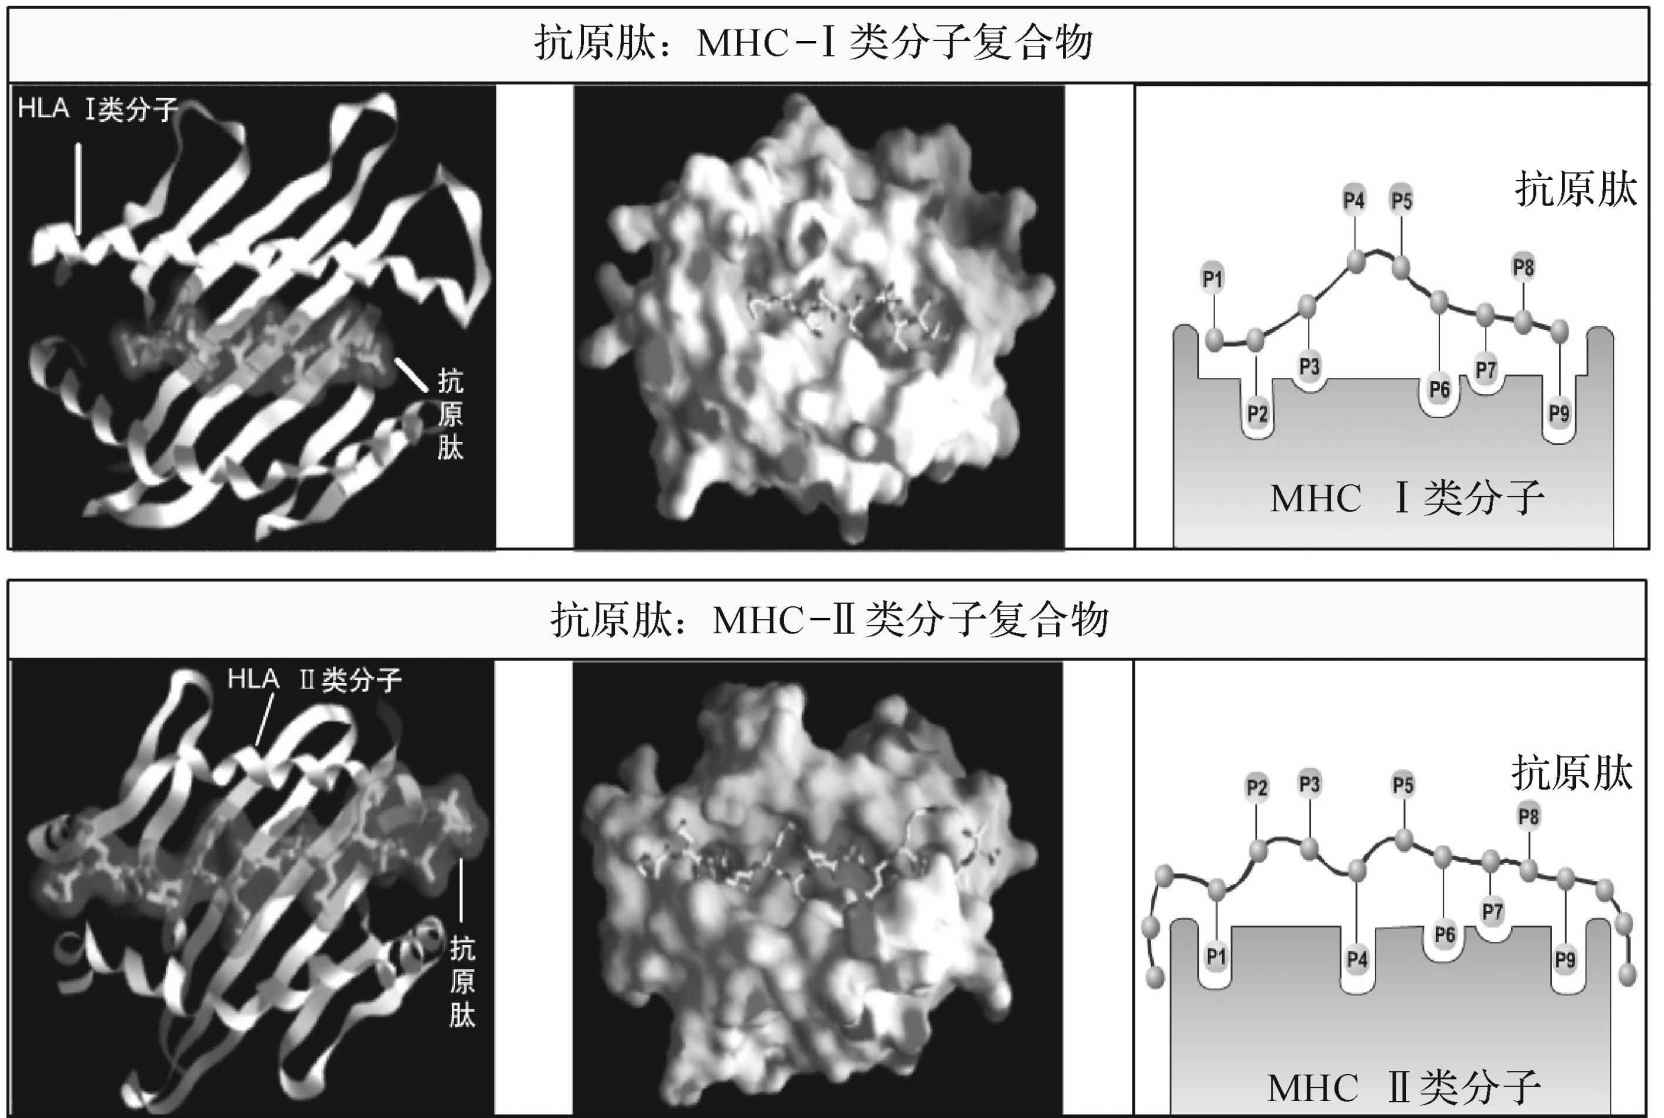
\includegraphics[width=.6\textwidth]{./images/Image00108.jpg}
 \captionsetup{justification=centering}
 \caption{抗原肽与MHC-I、II类分子结合示意图}
 \label{fig7-7}
  \end{figure} 

在抗原肽-MHC分子复合物中,抗原肽的两个或两个以上专司与MHC分子结合的氨基酸残基称为锚着残基(anchor
residue),MHC分子抗原结合槽与抗原肽锚着残基相对应的氨基酸残基称为锚着位(pocket)。

(二)参与T细胞限制性识别

TCR在识别抗原肽的同时,还须识别与抗原肽结合的同基因型MHC分子,此即MHC限制性(MHC
restriction)(图\ref{fig7-8})。CD8\textsuperscript{+}
T细胞在识别抗原肽的同时,须识别MHC-Ⅰ类分子,此为MHC-Ⅰ类限制性;CD4\textsuperscript{+}
T细胞在识别抗原肽的同时,须识别MHC-Ⅱ类分子,此即MHC-Ⅱ类限制性。

\begin{figure}[!htbp]
 \centering
 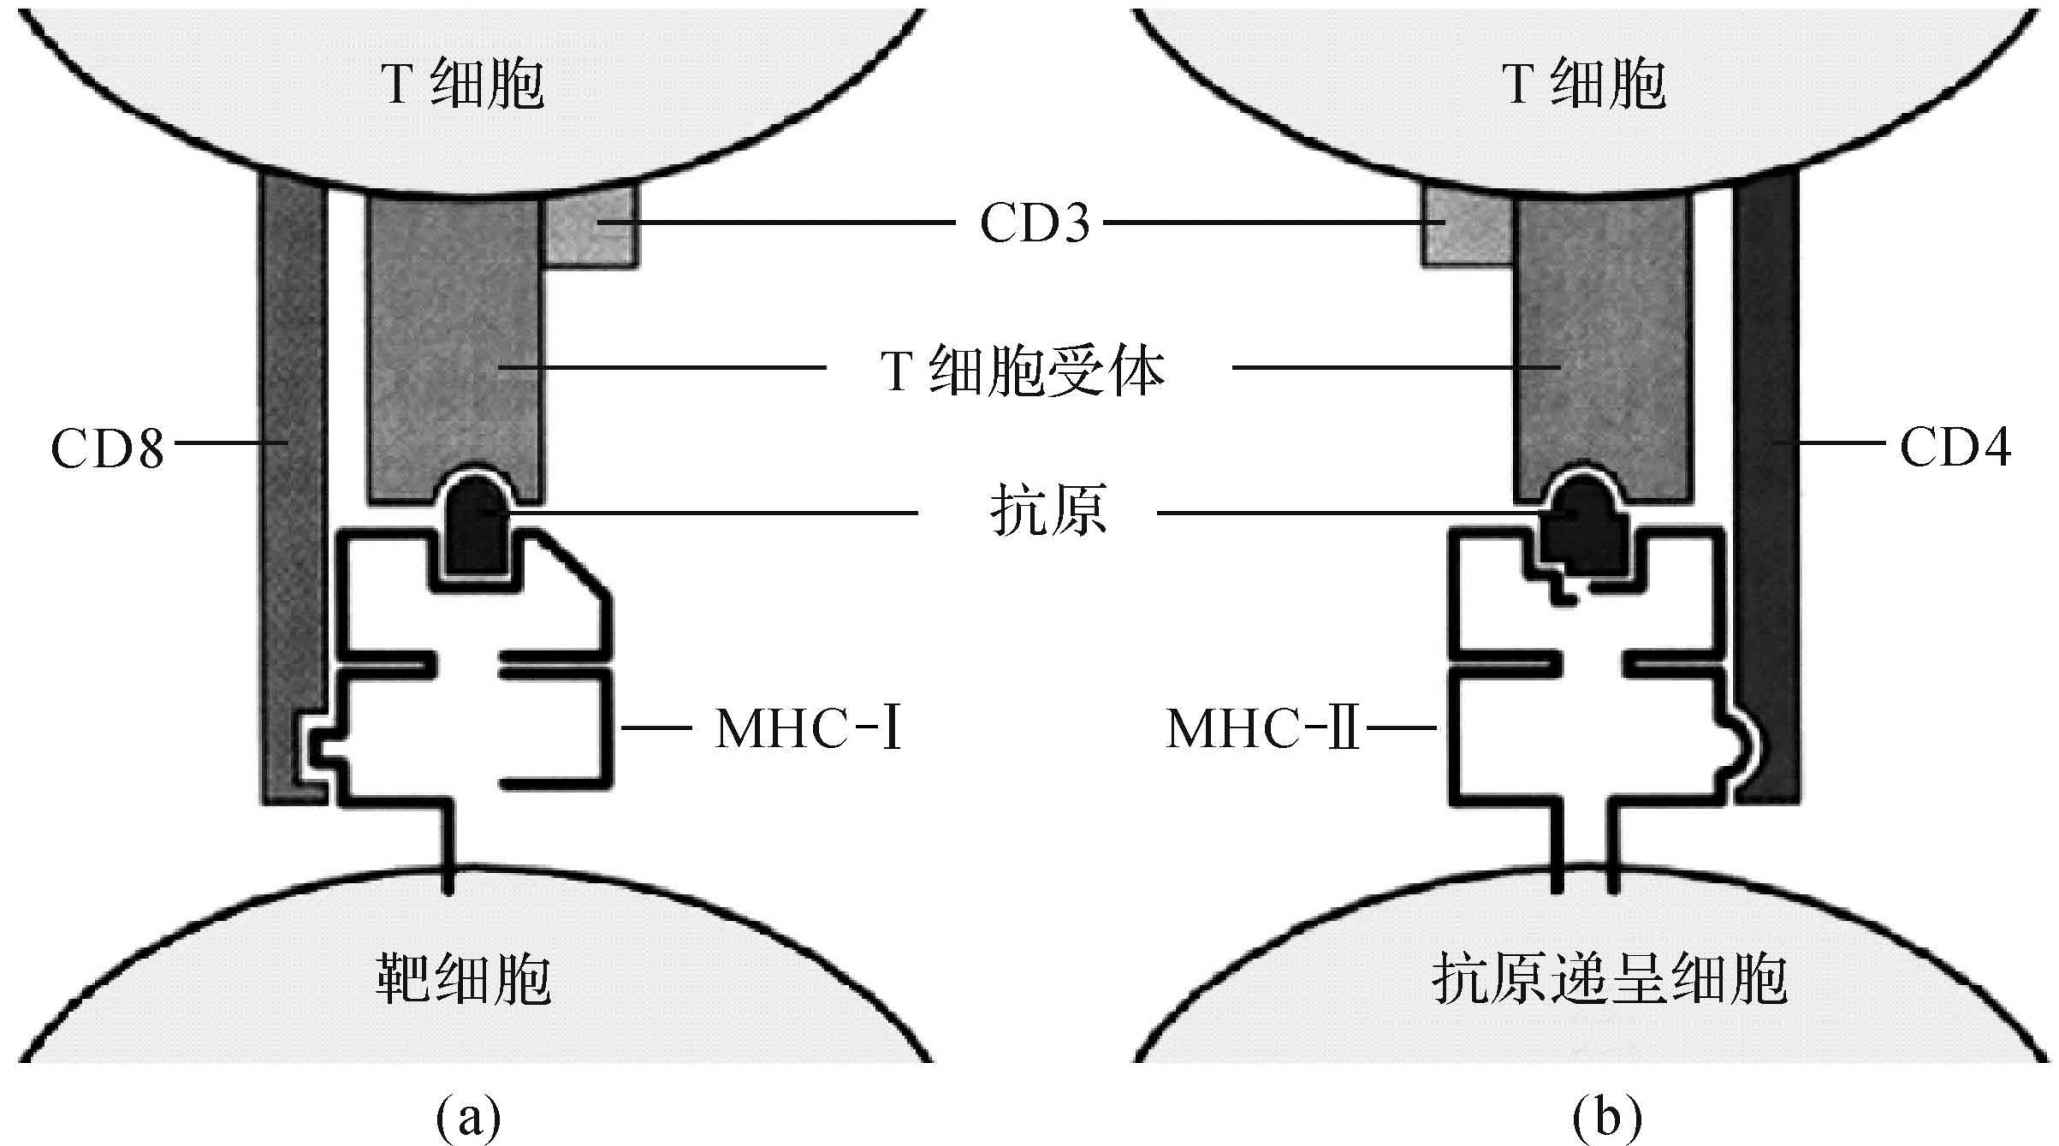
\includegraphics[width=.6\textwidth]{./images/Image00109.jpg}
 \captionsetup{justification=centering}
 \caption{MHC限制性}
 \label{fig7-8}
  \end{figure} 

(三)参与T细胞在胸腺的发育

T细胞在胸腺中的发育涉及复杂的选择过程,无论是阳性选择或阴性选择,均有赖于MHC-Ⅰ类和Ⅱ类分子参与。

(四)诱导同种移植排斥反应

同种异型MHC分子是介导移植排斥反应的关键分子,供、受者间MHC不匹配可导致移植排斥反应。

\section{HLA与医学实践}


\subsection{HLA与同种器官移植}

同种异体间器官移植(尤其是造血干细胞移植)的成败在很大程度上取决于供、受者间HLA型别的差异,即组织相容程度。因此,移植术前进行HLA配型成为寻找合适供者的主要依据。另外,建立造血干细胞捐赠者资料库(或脐带血库)并在需要时从中筛选供者,有赖于HLA
分型。


\subsection{HLA与疾病关联}

迄今已发现50余种人类疾病(多为免疫相关性疾病)与HLA关联(association),即携带某型HLA的个体比不携带此型别的个体易患(或不易患)特定疾病(表\ref{tab7-2})。典型的例子是:约90\%强直性脊柱炎患者携带HLA-B27,而正常人群则仅为9\%。

\begin{longtable}[]{@{}lll@{}}
    \caption{与HLA呈现强相关的一些自身免疫病}
    \label{tab7-2}\\
\toprule
疾病 & HL A 抗原 & 相对风险(% )\tabularnewline
\midrule
\endhead
强直性脊柱炎 & B27 & 59.8\tabularnewline
急性前葡萄膜炎 & B27 & 10.0\tabularnewline
肾小球性肾炎咯血综合征 & DR2 & 15.9\tabularnewline
多发性硬化症 & DR2 & 4.8\tabularnewline
乳糜泻 & DR3 & 10.8\tabularnewline
甲状腺功能亢进 & DR3 & 3.7\tabularnewline
重症肌无力 & DR3 & 2.5\tabularnewline
系统性红斑狼疮 & DR3 & 5.8\tabularnewline
胰岛素依赖性糖尿病 & DR3 /DR4 & 25.0\tabularnewline
类风湿性关节炎 & DR4 & 4.2\tabularnewline
寻常天疱疮 & DR4 & 14.4\tabularnewline
淋巴瘤性甲状腺肿 & DR5 & 3.2\tabularnewline
\bottomrule
\end{longtable}

HLA与疾病相关的程度可用相对危险性(relative
risk,RR)表示,RR数值越大,与疾病的相关性越强(RR>3表示有较强相关性)。

同一基因座上HLA等位基因的差别可导致个体对某些疾病具有易感性或抗性。与HLA
关联的疾病多为自身免疫病,提示HLA
等位基因的差别可导致免疫应答类型与效应的不同。HLA
与疾病关联的机制目前尚未完全阐明,多数证据提示此与HLA
分子递呈致病性抗原肽或影响T细胞识别有关。


\subsection{HLA分子表达异常与疾病的发生}

1.HLA-Ⅰ类分子表达降低与恶性肿瘤:肿瘤细胞所表达的HLA-Ⅰ类分子在CD8\textsuperscript{+}
CTL应答中具有重要作用。目前已发现,许多恶性肿瘤细胞其HLA-Ⅰ类分子表达减弱或缺失,导致CD8\textsuperscript{+}
T细胞的MHC限制性识别发生障碍,使肿瘤逃避免疫监视。实验研究证明,增强肿瘤细胞HLA-Ⅰ类分子表达,可促进CTL杀瘤效应,从而有效遏制肿瘤生长和转移。

近年还发现,某些病毒(如HIV)感染的宿主细胞,其HLA-Ⅰ类分子的表达也降低,这可能是病毒逃避机体免疫攻击的机制之一。

2.HLA-Ⅱ类分子异常表达与自身免疫病:
HLA-Ⅱ分子主要表达于抗原递呈细胞表面。已发现,某些自身免疫病靶器官的组织细胞可异常表达HLA-Ⅱ类分子,从而有可能将自身抗原递呈给免疫细胞,使之激活,产生异常自身免疫应答,导致自身免疫病。


\subsection{HLA分型在法医学中的应用}

由于HLA
具有极为复杂的多态性,且HLA复合体中所有基因均为共显性表达并以单元型形式遗传,从而奠定了其应用于法医学实践的理论基础:①无亲缘关系的个体间,其HLA等位基因完全相同的几率几乎为零;②HLA是伴随个体终生的遗传标志。据此,HLA
分型技术已成功地应用于法医学领域的亲子鉴定与个体识别。

\noindent\textbf{【理解与思考】}

1.请你形象地述说经典的HLA-Ⅰ、Ⅱ、Ⅲ类基因所编码的产物在整个机体防御体系中的作用。

2.结合遗传学知识,说明不同个体同一基因座位上的基因存在差别所导致的多态性的机理。

\noindent\textbf{【课外拓展】}

1.除了主要组织相容性抗原,还有哪些次要组织相容性抗原?

2.MHC是如何发现的?在参与抗原递呈加工中有哪些作用?

3.MHC-Ⅰ类和Ⅱ类分子是如何参与淋巴细胞阳性选择或阴性选择的?

\noindent\textbf{【课程实验与研究】}

1.如何检测细胞表面MHC的种类及其活性?

2.如何从基因的角度,研究MHC的表达与疾病的关联?

3.检测与治疗免疫相关性疾病的主要原则是什么?

4.提出一种假设与方案,使两个HLA差异很大的个体能进行器官移植。

\noindent\textbf{【课程研讨】}

1.HLA与疾病有哪些关系?

2.哪些因素会影响器官移植成功与否?

3.如果细胞MHC表达过强或过弱会导致怎样的结果?为何?

4.你认为MHC的研究热点是什么?要解决什么问题?

\noindent\textbf{【课后思考】}

1.MHC的概念。

2.HLA-I、II类抗原分子的结构、分布及其主要功能、特征。

3.MHC的发现与研究,对免疫学的发展有何意义?

\noindent\textbf{【课外阅读】}
\begin{center}
    \textbf{\Large HLA-Ⅰ类分子异常表达与肿瘤免疫逃逸}
\end{center}

\begin{center}
    {\large 一、肿瘤中HLA-I类分子缺失和下调的表型及其分子机制}
\end{center}

肿瘤的早期发生常常存在于免疫功能正常的机体中。由于HLA基因控制着T细胞以及NK细胞介导的免疫应答中心分子的功能,肿瘤细胞往往“借用”各种HLA-Ⅰ类分子下调或缺失的表型来逃避机体的免疫监视。针对各种类型提高其HLA-I类分子的表达从而恢复机体对肿瘤细胞的识别和杀伤的手段也各异。

1.HLA-Ⅰ类分子的完全缺失

HLA-Ⅰ类分子的完全缺失能使肿瘤细胞逃避CTL的攻击,但有可能被NK细胞所杀伤。因为NK细胞上存在一些抑制性受体(KIR)需要结合某些HLA-I类分子而抑制其活性,所以HLA-Ⅰ类分子完全缺失的肿瘤细胞有可能使NK细胞活化而被杀伤,这就是“missing
self”学说的主要观点:轻链β\textsubscript{2}
M基因缺陷是HLA-Ⅰ类抗原完全缺失的主要原因。因为β\textsubscript{2}
M基因含有一些重复序列,在错配修复障碍的基因型个体中容易成为受影响的靶点,所以在微卫星不稳定(MMP)的结肠癌和胃癌中β\textsubscript{2}
M的基因突变最为常见。β\textsubscript{2}
M基因缺陷包括表达缺失或功能缺陷。已在人类肿瘤中发现了β\textsubscript{2}
M基因的大片段缺失或是点突变,这大多会抑制β\textsubscript{2}
M基因mRNA的翻译,导致转录水平的表达缺失。而最近发现的β\textsubscript{2}
M基因一个点突变即改变了β\textsubscript{2}
M蛋白第25位氨基酸,破坏了β\textsubscript{2}
M蛋白天然结构中的二硫键,使之不能与HLA-Ⅰ类重链结合而使表面HLA-Ⅰ类复合物完全缺失。β\textsubscript{2}
M基因中的突变热点是外显子1中的CT重复序列。据统计,肿瘤细胞存在HLA-Ⅰ类抗原的完全缺失中有75\%都存在这个区域的点突变。β\textsubscript{2}
M基因缺陷通常不能被IFN-γ处理所恢复,只能转入野生型的β\textsubscript{2}
M基因使HLA-Ⅰ类分子得以表达。这一类型的患者不适宜T细胞介导的免疫治疗。但是,由于β\textsubscript{2}
M基因突变导致HLA-I类抗原的完全缺失需要“二次突变”,即一对等位基因中一个发生突变而另一个发生缺失使两者都失活,因此这种完全缺失类型的发生频率要比其他类型都低。

2.HLA-Ⅰ类分子表达下调

根据“Missing
self”的学说,肿瘤细胞上的HLA-Ⅰ类分子缺失能活化NK细胞的KIR受体而被其杀伤。但是HLA-Ⅰ类分子的下调如果既能达到不激活CTL,但同时仍能抑制NK细胞的量,反而有可能同时抑制NK和CTL的活性。这是最普遍的存在于各种肿瘤细胞中的类型,其分子机制也最为多样和复杂,也是人们研究的热点。

HLA-Ⅰ类分子的下调可由TAP、LMP分子表达减少或者功能异常造成。尽管存在非蛋白酶体的蛋白水解途径和非TAP依赖性的抗原递呈途径,这一类型细胞HLA-Ⅰ类分子的表达仍然很低。到目前为止,蛋白酶体亚单位LMP2、7、10究竟是组成性表达还是IFN-γ诱导性表达以及它们对于抗原加工递呈过程来说是否必不可少仍有争论。但是,可以肯定的是,这些亚单位能增强一些特定的蛋白酶体的活性,这些蛋白酶降解产生的肽段更倾向于结合重、轻链以形成HLA-Ⅰ类分子复合体。因此这些蛋白质的改变必定会影响到肿瘤细胞递呈HLA-Ⅰ类分子的质与量,影响到肿瘤被机体免疫系统识别和杀伤的可能性。

HLA-Ⅰ类分子的总体下调和丢失还可由于重链基因的表达减少所至。HLA-Ⅰ类重链转录直接受转录起始点上游调节区URR(Upstream
Regulatory
Region)调节,通过其中的顺式作用元件和反式作用因子的相互作用来实现。HLA-Ⅰ类基因重链在5'启动子区含有CpG岛。首先在滋养层上皮起源的细胞系中发现了HLA-Ⅰ类分子表达受到其重链甲基化程度的影响。近年来,由于重链启动子区的DNA甲基化、乙酰化等表遗传因素影响到启动子区的染色体结构导致HLA-Ⅰ类重链转录减少已经在许多肿瘤的研究中被报道。这样的肿瘤细胞往往对TNF-α和IFN-γ等细胞因子的处理无反应,只有通过5-杂氮胞苷的去甲基化处理才能使HLA-Ⅰ类分子表达上调,恢复对CTL杀伤的敏感性。但由于这类药物的毒性和副作用太大,其临床应用受到很大程度的限制。

3.HLA-I类分子单体型的缺失

如缺失一条染色体上连锁的HLA-A2,B7,Cw7基因。这种缺失往往发现于对HLA分子分型或对HLA基因区域进行杂合性丢失检测时。宫颈癌中约有50\%病例存在这种缺失,在其他肿瘤中也发现有不同程度的HLA-Ⅰ类抗原单体型的缺失。在细胞分裂过程中染色体异常分离造成第6号染色体短臂中部分片段缺失是发生这种情况的主要原因。在肿瘤中已发现不同类型的染色体重组伴随各种6P21.3区片段的缺失。单体型的缺失同样不能被IFN-γ处理所恢复。

4.位点特异性HLA-Ⅰ类分子表达下调和缺失

可由位点特异性单抗检测出。在黑色素瘤组织及黑色素瘤细胞系中已经发现了明显的HLA-B位点的表达下调。随着位点特异性抗体的不断产生,这一类表型的检出率明显增加。

5.HLA-Ⅰ类分子等位基因选择性下调或丢失

如果HLA-A2分子缺失,这通常是因为编码HLA重链的基因缺失或突变抑制了其转录和翻译的效率造成。由于HLA重链基因的高度多态性,与β2M基因突变相比,这只须“一次突变”造成一种杂合性的等位基因背景即可。但与β2M基因突变不同的是在HLA重链基因中尚未找到发生突变的热点区域。

6.复合型表型

通常由上述两种或两种以上的表型混合存在而形成,这使得肿瘤细胞表面HLA-Ⅰ类分子异常表达的形式更为复杂多样。

7.干扰素无反应性表型

有一些肿瘤细胞基础性的HLA-Ⅰ类分子的表达是正常的,但经干扰素处理后无反应。这种类型的肿瘤往往存在干扰素信号传导通路上的缺陷,临床运用干扰素治疗往往无效。

8.经典的HLA-I类分子缺失或下调,非经典的HLA-Ⅰ类分子表达增加

在一个特定的肿瘤中活化T细胞和激活NK细胞的HLA-Ⅰ类等位基因可能不同,因此在肿瘤细胞表面表达哪种HLA-Ⅰ类分子,表达量的多少决定了它被CTL和NK识别杀伤的可能性。从这个角度来说,HLA-Ⅰ类抗原选择性下调和丢失较HLA-Ⅰ类抗原总体改变更易于逃逸免疫监视。如HIV-1的nef蛋白可抑制HLA-Ⅰ类分子A和B位点的表达,而不影响NK细胞的作用靶点HLA-Ⅰ类分子C和E位点的表达。只要恢复HLA-A和B位点的表达就可以打破这种免疫耐受,使肿瘤细胞被机体免疫系统重新识别。因此,了解某一个体肿瘤细胞的HLA-Ⅰ类分子具体表型及其分子机制,对于临床免疫治疗手段的选择是非常重要的。

\begin{center}
    {\large 二、T细胞的克隆选择学说及其对肿瘤细胞HLA-Ⅰ类分子改变的决定性作用}
\end{center}

肿瘤中HLA-Ⅰ类分子表达缺失或下调的表型复杂多样,具有肿瘤特异性和个体特异性。肿瘤细胞是如何获得这种多变的HLA-Ⅰ类分子缺失表型的呢?在肿瘤发生的早期,往往机体的免疫功能还未得到破坏,肿瘤还处于机体的免疫监视下。由于肿瘤基因的不稳定,在原发癌中,往往突变产生很多具有不同HLA-Ⅰ类分子表达类型的多个克隆。T细胞识别杀伤一些HLA-Ⅰ类表达正常的肿瘤克隆,而一些HLA-Ⅰ类表达缺陷的克隆得以逃避免疫杀伤生存下来,而这些克隆往往出现于后期的复发或转移瘤中。肿瘤细胞的自身变化和T细胞对于肿瘤的选择压力使得HLA-I类分子的表达在肿瘤进程中处于动态变化。

\begin{center}
    {\large 三、肿瘤免疫}
\end{center}

机体针对肿瘤的免疫监视学说很早就被人们提出,后来在临床与实践中有很多证据支持。如儿童和幼儿患肿瘤较少,而在免疫系统衰退的老年人中肿瘤发病率很高。在实体瘤中也可以看到大量的淋巴细胞浸润,这是机体的细胞免疫识别杀伤肿瘤细胞的证据。然而T细胞的克隆选择学说及其对肿瘤细胞HLA-I类分子改变所起的决定性作用却没有充足的实验证据。直到2001年,Garcia-Lora小组才在小鼠实验中证实了这一假说的成立。实验者将H-2(小鼠HLA-I类分子)阴性的纤维肉瘤局部注射在免疫监视功能正常的BALB/C小鼠和无免疫功能的裸鼠局部,发现在这两组老鼠的肺部转移癌中H-2分子的表达截然不同。免疫监视功能正常的BALB/C小鼠肺转移癌H-2表达阴性,其参与HLA-Ⅰ类加工递呈的所有分子包括重链、轻链、TAP、LMP等加工分子全部表达下调。这种下调是IFN-γ处理可逆的,说明其改变发生在转录水平。而裸鼠转移癌H-2表达阳性。将两种转移癌再次分别注射入免疫功能正常的小鼠,只有来源于免疫监视功能正常的BALB/C小鼠肺转移癌才能形成肿瘤。而裸鼠肺转移癌因H-2表达阳性会被体内的免疫系统识别杀伤而没有肿瘤产生。这组实验充分体现了T细胞选择对肿瘤细胞HLA-Ⅰ类分子改变的决定性作用。

通过上述综述可以了解到在肿瘤细胞中HLA-Ⅰ类分子的表达不仅形式复杂多样,机制各异,而且在肿瘤与机体的相互“斗争”中处于不断的动态变化中。要改变HLA-Ⅰ类分子的异常表达,增强肿瘤的免疫原性使之被机体的免疫系统识别决非易事。但肿瘤细胞完整地表达MHC-I类分子是运用T细胞治疗肿瘤成功的先决条件,所以我们必须了解在不同的肿瘤中HLA-Ⅰ类分子表达情况及其分子机制,进行个体分析和分子诊断,才能有效地指导临床运用免疫治疗,提高免疫治疗的效果及成功率。随着免疫学研究的高速发展及研究方法不断进步,人们愈来愈发现HLA分子在肿瘤发生发展过程的复杂性与多样性。此过程中聚集着免疫学理论研究中的难点、重点和热点课题。而本课题的研究正是集中于肝癌这种特殊的HLA-Ⅰ类分子表达上调模型,着重于研究其分子机制。研究这一不同于其他肿瘤细胞HLA-Ⅰ类分子表达情况模型的确切机制将对肿瘤免疫学的认识起着重要作用,并对临床肿瘤免疫治疗提供理论依据。

